\section{Implementing a complete turn}
\label{sec:algorithms}

Consider a black pawn that reaches square 2 by jumping from 11. Three actions must occur in order: remove the captured piece, replace the pawn with a king, and check for a further jump by that king. The turn loop below also handles the simpler cases without allowing an invalid input to change sides.

\subsection{Main Control Loop and Turn Lifecycle}
\label{sec:game_loop}
Execution begins at \code{main} (\code{src/main.asm}, line~104). Before initializing the first board, \code{main\_arg\_check} inspects MARS's CLI program arguments (\code{\$a0 = argc}, \code{\$a1 = argv}). If \code{argv[0]} equals \code{"classic"}, \code{opt\_pretty} is cleared to \code{0}, activating the compact plain-board format required by automated transcript fixtures (\code{tests/test\_001..005}); otherwise, the game launches with the framed dual-panel board enabled by default (\code{opt\_pretty = 1}).

\begin{figure}[H]
\centering
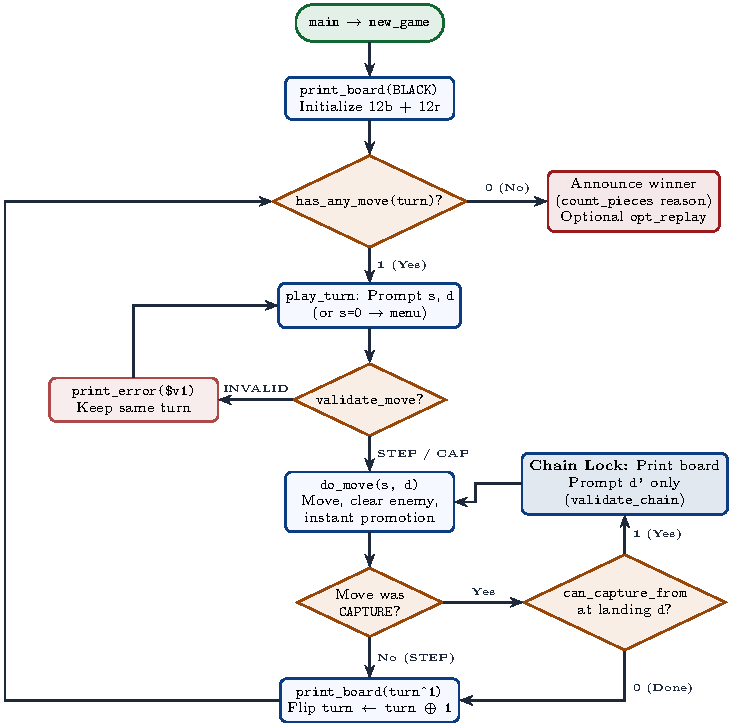
\includegraphics[width=0.96\textwidth]{figures/fig_fsm.pdf}
\caption{Main game loop and \code{play\_turn} finite-state control flow, highlighting invalid-move turn retention and the mandatory chain-capture lock loop.}
\label{fig:fsm}
\end{figure}

As depicted in Figure~\ref{fig:fsm}, \code{main\_loop} checks \code{has\_any\_move(turn)} \emph{before} every turn. If the active side has no legal move (either zero pieces or all pieces completely blocked), control branches to \code{main\_no\_moves}, announces the opponent as winner, and honors \code{opt\_replay}. Otherwise, \code{play\_turn} returns one of four status codes (\code{RESULT\_MOVED}, \code{RESULT\_RESTART}, \code{RESULT\_DRAW}, \code{RESULT\_QUIT}), and the turn flips (\code{xori \$t0, \$t0, 1}) strictly after a valid move (and any mandatory capture chain) completes.

\subsection{Move Classification and Validation Pipeline}
\label{sec:validation}
Rule checking in \code{src/rules.asm} is decomposed into three layered validators that return both a move classification in \code{\$v0} (\code{INVALID = 0}, \code{STEP = 1}, \code{CAPTURE = 2}) and a precise diagnostic code in \code{\$v1} (\code{ERR\_RANGE = 1} through \code{ERR\_BLOCKED = 11}):

\begin{enumerate}
    \item \textbf{\code{check\_start(s, side)}:} Verifies $1 \le s \le 32$ (\code{ERR\_RANGE}), checks that \code{square\_piece(s) != EMPTY} (\code{ERR\_EMPTY}), and confirms ownership via \code{is\_own} (\code{ERR\_NOT\_YOURS}). When \code{opt\_detail} or \code{opt\_hints} is active, \code{play\_turn} invokes \code{check\_start} immediately after the starting square is typed, rejecting bad starts before asking for a landing square.
    \item \textbf{\code{classify\_move(s, d, side)}:} Evaluates pure move geometry independent of global forced-capture rules:
    \begin{itemize}
        \item Validates starting square via \code{check\_start}, and landing square bounds $1 \le d \le 32$ (\code{ERR\_RANGE}) and vacancy \code{get\_cell(rd, cd) == EMPTY} (\code{ERR\_OCCUPIED}). Note that $s = d$ automatically fails here with \code{ERR\_OCCUPIED} because $s$ is already verified non-empty.
        \item Computes $\Delta r = r_d - r_s$, $\Delta c = c_d - c_s$, checks diagonal equality $|\Delta r| = |\Delta c|$ (\code{ERR\_NOT\_DIAGONAL}), extracts unit step signs $\text{sdr}, \text{sdc} \in \{-1, +1\}$, and checks \code{dir\_allowed} (\code{ERR\_BACKWARD}): kings (\code{'B'}, \code{'R'}) permit both signs; pawns require $\text{sdr} = -1$ for Black and $\text{sdr} = +1$ for Red.
        \item Dispatches distance checking: under standard English rules (\code{classify\_short}), $n = 1 \Rightarrow \code{STEP}$; $n = 2$ inspects midpoint $(r_s + \text{sdr}, c_s + \text{sdc})$ via \code{is\_enemy} (\code{CAPTURE} or \code{ERR\_NO\_ENEMY}); $n > 2 \Rightarrow \code{ERR\_TOO\_FAR}$. When \code{opt\_flying = 1} and \code{is\_king} holds, control branches to \code{classify\_flying} (Section~\ref{sec:advanced}).
    \end{itemize}
    \item \textbf{\code{validate\_move(s, d, side)} and \code{validate\_chain(s, d, side)}:} Both wrap \code{classify\_move}. If \code{classify\_move} returns \code{STEP}, \code{validate\_move} rejects it with \code{ERR\_MUST\_CAPTURE} whenever \code{opt\_forced = 1} and \code{side\_has\_capture(side) == 1}; similarly, \code{validate\_chain} unconditionally rejects \code{STEP} with \code{ERR\_CHAIN}, locking the player into continuing the capture sequence with the exact piece stored in \code{\$s1}.
\end{enumerate}

\subsection{Execution, Instant Promotion, and Immediate Backward Chain Capture}
\label{sec:promotion_chain}
A subtle and explicitly graded requirement in Section~1.2.4 (Figure~8) of the CO2008 specification states: \emph{``If a pawn advances to the final row via a capture, it is instantly promoted to king and can immediately chain capture backwards.''} In our implementation, this behavior emerges cleanly from the exact sequencing between \code{do\_move} (\code{src/rules.asm}, lines~507--566) and \code{play\_turn\_captured} (\code{src/main.asm}, lines~288--348):

\begin{lstlisting}[style=mipsstyle, caption={Unified intermediate-square clearing, instant promotion (\code{src/rules.asm}:528--560), and post-promotion chain check (\code{src/main.asm}:295--298).}, label={lst:domove_chain}]
    # --- src/rules.asm: do_move(a0 = s, a1 = d) ---
    sub  $t3, $v0, $s1            # dr = rd - rs
    sub  $t4, $v1, $s2            # dc = cd - cs
    li   $t5, 8                   # stride = sdr * 8 + sdc in {-9, -7, +7, +9}
    bgtz $t3, do_move_dc
    li   $t5, -8
do_move_dc:
    addi $t5, $t5, 1
    bgtz $t4, do_move_clear
    addi $t5, $t5, -2
do_move_clear:                    # clears jumped enemy (works for both 2-step & Flying King)
    add  $t0, $t0, $t5
    beq  $t0, $t1, do_move_promote
    sb   $t2, board($t0)          # $t2 = EMPTY ('0')
    j    do_move_clear
do_move_promote:                  # promote IMMEDIATELY upon landing on row 0 or row 7
    li   $t6, 0
    bne  $s3, PAWN_BLACK, do_move_red
    bnez $v0, do_move_ret         # Black promotes at rd == 0
    li   $t7, KING_BLACK
    sb   $t7, board($t1)
    li   $t6, 1
    j    do_move_ret
do_move_red:
    bne  $s3, PAWN_RED, do_move_ret
    bne  $v0, 7, do_move_ret      # Red promotes at rd == 7
    li   $t7, KING_RED
    sb   $t7, board($t1)
    li   $t6, 1
    # --- src/main.asm: play_turn_captured (runs right after do_move) ---
    move $a0, $s1                 # $s1 = landing square; board[$s1] already holds 'B' or 'R'
    move $a1, $s3                 # $s3 = current side
    jal  can_capture_from         # checks all 4 diagonals for newly crowned king
\end{lstlisting}

Notice two architectural highlights in Listing~\ref{lst:domove_chain}:
\begin{itemize}
    \item \textbf{Single-loop capture clearing:} Computing the flat-array diagonal stride $\$t5 = 8\cdot\text{sdr} + \text{sdc} \in \{-9, -7, +7, +9\}$ lets the same 4-instruction loop clear a standard 1-square jump or an arbitrary-distance Flying King capture with zero branch divergence.
    \item \textbf{Zero special-case promotion chain logic:} Because \code{do\_move} writes \code{KING\_BLACK} or \code{KING\_RED} into \code{board[\$t1]} \emph{before} \code{play\_turn\_captured} calls \code{can\_capture\_from(\$s1, \$s3)}, \code{can\_capture\_from} reloads the newly crowned king from \code{board}, sees \code{dir\_allowed == 1} for both $dr = -1$ and $dr = +1$, and seamlessly prompts for backward chain jumps.
\end{itemize}

Figure~\ref{fig:promo_chain} illustrates both verified promotion-chain scenarios: Specification Figure~8 (\code{15x24 24x31 31x22 22x13}, verified by \code{test\_rules.py}) and fixture \code{test\_001} (\code{11x2 2x9 9x18}, recommended in \code{README.md} for oral defense).

\begin{figure}[H]
\centering
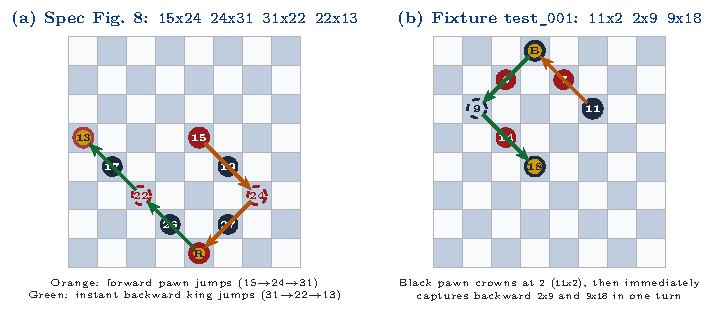
\includegraphics[width=0.96\textwidth]{figures/fig_promo_chain.pdf}
\caption{Instant promotion followed by immediate backward chain captures in (a) Specification Figure~8 and (b) full-game benchmark \code{test\_001}.}
\label{fig:promo_chain}
\end{figure}

\subsection{Win-Condition Detection (Elimination and Trapping)}
\label{sec:win_detect}
Instead of merely counting remaining pieces, \code{has\_any\_move(side)} (\code{src/rules.asm}, lines~566--623) packs the 32 dark squares into three 32-bit bitboards (\code{BP}, \code{RP}, \code{K}) via \code{pack\_bitboards} and evaluates all 32 squares in parallel using our 3-shift Chinook SWAR step operators (\code{swar\_up\_steps}, \code{swar\_dn\_steps}) followed by the SWAR capture kernels (\code{swar\_up\_caps}, \code{swar\_dn\_caps}). This single $O(1)$ bit-parallel predicate handles \emph{both} victory conditions uniformly:
\begin{itemize}
    \item \textbf{Piece Elimination:} When zero friendly pieces exist (\code{UP = DN = 0}), every SWAR test short-circuits immediately and returns \code{0}.
    \item \textbf{Complete Blockade / Trapping (Specification Fig.~9):} Even when friendly pieces remain (e.g., \code{test\_003} with 1 Red pawn left, \code{test\_004} with 3 Black pawns left), if no bit lands in empty mask $E = \neg(\code{BP} \mid \code{RP})$ after either a single step or double-jump over an enemy, \code{has\_any\_move} returns \code{0}.
\end{itemize}
When pretty mode or detailed messages are enabled, \code{main\_loss\_reason} invokes \code{count\_pieces(turn)}---accelerated by branchless 32-bit SWAR Hamming weight (\code{popcount} (Warren, \emph{Hacker's Delight}, Sec.~5-1))---to distinguish \code{"<Side> has no pieces left."} from \code{"<Side> has no legal moves left."}. Furthermore, two formal invariants hold across all rule variants:
\begin{enumerate}
    \item Under \code{opt\_forced = 1}, a player has a legal move if and only if they have a capture \emph{or} (having no capture) a legal step---logically identical to $\text{SWAR\_Step} \lor \text{SWAR\_Cap}$.
    \item \textbf{Mobility Equivalence Theorem (Flying Kings):} Under \code{opt\_flying = 1}, a flying king can capture an enemy at distance $k \ge 2$ \emph{only if} the adjacent diagonal cell at distance $k = 1$ is empty, which already guarantees a legal distance-1 step! Consequently, \code{has\_any\_move} is \emph{mathematically identical} for both standard and flying kings, allowing the $O(1)$ SWAR path to execute unconditionally (verified across 50,000 randomized side-boards with 0 exceptions).
\end{enumerate}

\subsection{Fault-Tolerant Buffered Input Subsystem}
\label{sec:input_parser}
Standard MARS student implementations rely on \code{syscall 5} (\code{read\_int}), which throws an unrecoverable runtime exception whenever the user types letters, blank lines, or overflowing integers. To guarantee zero crashes under adversarial input and clean termination on piped CLI EOF, \code{src/board\_io.asm} implements a three-layer input parser built on \code{syscall 14} (\code{read} from \code{fd = 0}):
\begin{enumerate}
    \item \textbf{\code{read\_input\_line()}:} Maintains a 256-byte chunk buffer (\code{input\_chunk}) with cursors \code{input\_next} and \code{input\_end} so unread bytes after a newline persist across calls. It copies up to \code{INPUT\_SIZE = 64} bytes into \code{input\_line}, gracefully drains overlong lines ($> 63$ characters) up to the next \code{'\textbackslash n'} so subsequent reads stay synchronized, strips trailing \code{'\textbackslash r'} (handling exact 63-char + CRLF lines without false rejection), treats a final line without \code{'\textbackslash n'} as valid, and returns \code{INPUT\_END = -2} on true EOF.
    \item \textbf{\code{read\_number()}:} Skips leading spaces/tabs, parses ASCII digits while clamping values $\ge 1000$ to \code{9999} (preventing 32-bit signed integer overflow on inputs like \code{99999999999999999999}), skips trailing whitespace, and validates that the cursor reached the exact returned byte length \code{\$t3 = input\_line + len}---a subtle safeguard that rejects embedded NUL bytes such as \code{"21\textbackslash 0x"}. Any malformed input returns \code{INPUT\_INVALID = -1}.
    \item \textbf{\code{read\_square(side)}:} Calls \code{read\_number()} and maps $1 \dots 32$ through \code{view\_square(val, side)}, transparently translating Red's relative coordinates while leaving \code{0} (menu trigger), \code{-1}, and \code{-2} untouched.
\end{enumerate}
